\documentclass[a4paper]{article}

\usepackage[utf8]{inputenc}
\usepackage[portuges]{babel}
\usepackage{a4wide}
\usepackage{graphicx}

\title{Projeto de Laboratórios de Informática 1\\Grupo 044}
\author{Miguel Brandão (A82349) \and Vítor Gomes (A75362)}
\date{\today}

\begin{document}

\maketitle

\begin{abstract}
 

  Este documento é o relatório do projeto de Laboratórios de Informática, \emph{Bomberman}, do Mestrato Integrado em Engenharia Informática da Universidade do Minho.
  Neste documento explicita-se o trabalho desenvolvido para a implementação do projeto, constituído por 6 tarefas. Para as tarefas de maior importância, explica-se a linha de raciocinio e a forma de como as tarefas foram implementadas.
\end{abstract}

\tableofcontents

\section{Introdução}
\label{sec:intro}

Neste relatório apresenta-se um relato sobre o desenvolvimento do projeto
para a unidade curricular de Laboratórios de Informática 1 (LI1),
do Mestrado Integrado em Engenharia Informática da Universidade do Minho.
Este projeto era a implementação de um jogo (Bomberman) utlizando a linguagem
de programação funcional Haskell.
Para este efeito, o projeto foi dividido em 6 tarefas.

Estas tarefas consistiam na implementação de um mecanismo gerador de mapas,
um módulo que altere o estado do jogo em conformidade com o comando de um
jogador (secção~\ref{tarefa2}), um mecanismo de compressão / descompressão
que permita comprimir o estado do jogo (secção~\ref{tarefa3}), um módulo
capaz de reagir à passagem do tempo (secção~\ref{tarefa4}), criação de
do jogo e interface gráfica agregando as tarefas anteriores e utilizando a
biblioteca \texttt{Gloss} (secção~\ref{tarefa5}) e, ainda, implementar uma estratégia de combate
para criar um \textit{bot} que jogue Bomberman automaticamente (secção~\ref{tarefa6}).


\section{Tarefa 2}
\label{tarefa2}

A \emph{tarefa 2} consiste em, dada uma descrição do estado de jogo e um comando de um dos jogadores, determinar o efeito desse comando no estado do jogo. Os comandos possíveis são:

\begin{tabular}[c]{lll}
U & Up & (o jogador move-se para cima) \\
D & Down & (o jogador move-se para baixo) \\
R & Right & (o jogador move-se para a direita) \\
L & Left & (o jogador move-se para a esquerda) \\
B & Bomb & (o jogador coloca uma bomba)
\end{tabular}

Assim, foram implementadas funções para modificar o estado de jogo de acordo com o comando do jogador, que seguem as seguintes regras:
\begin{enumerate}
  \item Um jogador não se pode mover para um bloco de pedra nem para um tijolo.
  \item Um jogador não pode colocar uma bomba num local onde já esteja uma.
  \item Um jogador não pode colocar um número superior de bombas ao permitido pelo número de powerups "Flames" que apanhou.
  \item Quando colocada, a bomba tem de ser representada na estado de jogo depois dos powerups e antes dos jogadores, com a coordenada y ordenada por ordem crescente e, caso a coordenada y de duas bombas seja igual, com a coordenada x ordenada por ordem crescente.
  \item Se um jogador se mover para a posição de um powerup destapado, "apanha" esse powerup.
  \item Quando um jogador apanha um powerup, este deve ser eliminado do mapa e adicionado no fim da string que representa o jogador, sendo os powerups ordenados de forma a que os powerups "Flames" (!) sejam colocados depois dos powerups "Bombs" (+).
  \item O raio da bomba é definido pela quantidade de powerups "Flames" que o jogador apanhou até ao momento em que coloca a bomba, seguindo a fórmula \(1+f\), sendo \(f\) o número de powerups "Flames" que o jogador apanhou até ao momento em que coloca a bomba.
\end{enumerate}


\section{Tarefa 3}
\label{tarefa3}

O objetivo a atingir com a \emph{tarefa 3} era a compressão e descompressão
do estado do jogo de forma a que seja possível gravar o estado de jogo num
formato menos espaçoso e recuperar o estado de jogo inicial.
Para a resolução deste problema implementou-se várias estratégias de redução
do estado do jogo, estas foram:
\begin{enumerate}
  \item Eliminação de todos os blocos do tipo pedra e os espaços vazios nos cantos do mapa
  \item Substiuição de caracteres seguidos repetidos
  \item Conversão de todos os números por um caracter
  \item Representação dos power ups no mapa
\end{enumerate}

A implementação da 1ª estratégia foi uma das que maior impacto fez na redução do tamanho do
estado do jogo e, para que mais tarde fosse possível recuperar os blocos removidos, bastava
apenas ter conhecimento do tamanho do mapa original.

A 2ª estratégia passou por substituir a representação caracteres iguais repetidos por apenas
um caracter e o número de vezes que esse caracter é repetido, ou seja, \texttt{"????"} seria
subsituído por \texttt{"4?"}.

Com a implementação da 3ª estratégia, para além reduzir o tamanho dos números com mais
de 1 algarismo, foi possível retirar os espaços entre algumas informações, por exemplo,
entre as coordenadas dos jogadores

A última estratégia é implementada apenas em alguns casos, esta estratégia elimina a
necessidade de representar as coordenadas dos power ups ao representá-los no mapa por
um caracter que identifique o seu tipo e se está ou não descoberto. Contudo, esta estratégia
aumenta o tamanho em certos casos pois pode diminuir bastante a eficácia da 3ª estratégia.
Para resolver este problema, os tamanhos do estado do jogo com e sem a implementação do 4º
método são comparados e é selecionado o estado do jogo mais curto e atribuído um caracter
identificador das estratégias utilizadas para que o estado de jogo possa ser descomprimido
corretamente.



\section{Tarefa 4}
\label{tarefa4}

A \emph{tarefa 4} consiste em, dada uma descrição do estado de jogo e o número de instantes de tempo restantes do jogo, determinar o efeito da passagem de um instante de tempo (\emph{tick}) nesse estado. Para tal ser conseguido, era necessário manipular as \emph{bombas}, mais propriamente os seus \emph{ticks}, representar os seus efeitos e despoletar um \emph{efeito caracol} quando quando faltassem \((n-2)^2\) ticks\footnote{\(n\) = dimensão do mapa}.

\subsection{Estruturas de Dados}
\label{dadosT4}

Para facilitar a alteração do estado do jogo, foi criado o data type \emph{DataEstado}:

\begin{verbatim}
data DataEstado = Mapa Int String
                | PowerUp Char Int Int
                | Bomba Int Int Int Int Int
                | Jogador Int Int Int Int Int
\end{verbatim}

Este data type permite identificar mais facilmente cada tipo de string (se é mapa, powerup, bomba ou jogador) e facilita a alteração de um ou vários valores através do \emph{pattern matching}.

\begin{enumerate}
  \item Em \texttt{Mapa Int String}, \texttt{Int} é o número da linha do mapa, ou seja, a coordenada \emph{y} e \texttt{String} é a linha respetiva.
%    \begin{verbatim}
%>>>["#########","#  ??   #","# # # # #","# ?     #"]
%[Mapa 0 "#########",Mapa 1 "#  ??   #",Mapa 2 "# # # # #",Mapa 3 "# ?     #"]
%    \end{verbatim}
  \item Em \texttt{PowerUp Char Int Int}, \texttt{Char} é o identificador do powerup (+/!) e os seguintes \texttt{Int} são as coordenadas \emph{x} e \emph{y}, respetivamente.
\begin{verbatim}
>>>["+ 3 3","! 6 3"]
[PowerUp '+' 3 3,PowerUp '!' 6 3]
    \end{verbatim}
  \item Em \texttt{Bomba Int Int Int Int Int}, os \texttt{Int} são as coordenadas \emph{x} e \emph{y}, o número do jogador que colocou a bomba, o raio da bomba e os ticks que faltam para ela explodir, respetivamente.
\begin{verbatim}
>>>["* 4 3 0 3 1","* 3 7 1 1 1"]
[Bomba 4 3 0 3 1,Bomba 3 7 1 1 1]
    \end{verbatim}
  \item Em \texttt{Jogador Int Int Int Int Int}, o primeiro \texttt{Int} é o número do jogador e os seguintes \texttt{Int} são as coordenadas \emph{x} e \emph{y}, o número de powerups "Bombs" (+) que o jogador apanhou e o número de powerups "Flames" (!) que o jogador apanhou, respetivamente.
\begin{verbatim}
>>>["0 2 7 +!!","1 1 1"]
[Jogador 0 2 7 1 2,Jogador 1 1 1 0 0]
    \end{verbatim}
\end{enumerate}

\subsection{Implementação}
\label{implementacaoT4}

Para implementar a tarefa 4 era necessário, em primeiro lugar, de converter o estado de jogo de \texttt{[String]} para \texttt{[DataEstado]}. Tal conseguiu-se com a implementação da função
\begin{verbatim}
stringToDataEstado :: [String] -> Int -> [DataEstado]
\end{verbatim}

Para converter o estado de volta para \texttt{[String]}, de modo a poder ser usado pela função \texttt{avanca}, definiu-se a função
\begin{verbatim}
dataEstadoToString :: [DataEstado] -> [String]
\end{verbatim}

De seguida, foi necessário definir as funções que definem o comportamento das bombas, mais especificamente, da sua explosão, que deve obedecer às seguintes caraterísticas:
\begin{enumerate}
  \item Deve lançar chamas em todas as direções, de raio igual.
  \item Deve eliminar do estado de jogo todos os jogadores e powerups destapados que atingir.
  \item Se atingir outra bomba, o número de ticks que faltam para esta explodir passa para 1.
  \item As chamas não destroem os blocos de pedra que atingirem e são bloqueadas por estes.
  \item As chamas destroem os tijolos (?) que atingirem e são bloqueadas por estes.
  \item As chamas são bloqueadas pelos powerups.
\end{enumerate}

Posteriormente, definiram-se as funções que controlam o \emph{efeito caracol}, que obedecem às seguintes regras:
\begin{enumerate}
  \item O \emph{efeito caracol} começa quando faltarem \((n-2)^2\) ticks\footnote{\(n\) é a dimensão do mapa.} para o jogo acabar.
  \item Em cada instante de tempo "cai" um bloco de pedra. Quando tal acontecer, tudo o que está nessa posição deve ser eliminado.
  \item O \emph{efeito caracol} começa em (1,1) e deve continuar pelo eixo horizontal, da esquerda para a direita, até encontrar o limite da área jogável, altura em que deve continuar pelo eixo vertical, de cima para baixo, até voltar encontrar o limite da área jogável, continuando no eixo horizontal, da direita para a esquerda, até re-encontrar o limite da área jogável, continuando no eixo vertical, agora de baixo para cima, até encontrar o limite da área jogável, e assim sucessivamente.
\end{enumerate}

Por fim, definiu-se a função \texttt{avanca}, com o objetivo de unir todas as funções da Tarefa 4, concluindo-se assim esta tarefa. 


\section{Tarefa 5}
\label{tarefa5}

A \emph{tarefa 5} consistia em implementar o jogo usando a biblioteca \texttt{Gloss}.
Para isto, foi necessário definir um tipo que representasse todo o estado do jogo:

\begin{verbatim}
type Estado = (InformacaoMapa,[(Int,[Movimento])],Explosao,Coordenadas,
Imagens,Int,Janela,Opcoes)
\end{verbatim}

O tipo \texttt{InformacaoMapa} inclui toda a informação relativa aos elementos do mapa,
jogadores, power ups e bombas.
Esta informação é enviada no ínicio do jogo pela função criada na \emph{Tarefa 1} e
é atualizada ao longo do tempo através da função definida na \emph{Tarefa 4} (Secção \ref{tarefa4})
e do movimento dos jogadores (Secção \ref{movimento}).

O 2º elemento do estado guarda a informação relativa ao movimento atual de cada jogador
(\ref{movimento}).

O tipo \texttt{Explosao} contém as posições no mapa onde deverão ser desenhadas as explosões

O 4º elemento é um par de \texttt{Float} com o tamanho da janela, isto foi necessario para
fazer com que o desenho do estado do jogo aumentasse ou diminuisse consoante se aumenta ou
diminui a janela do jogo.

No 5º e 6º elementos localizam-se, respetivamente, as imagens importadas e o tick atual do jogo.

O 7º elemento define em que momento está o programa, isto é, no menu das opções, no decorrer
do jogo ou no ecrã de vitória. Este elemento é reservado a um tipo de dados definido por:

\begin{verbatim}
data Janela = MenuPrincipal | Jogo | Fim
\end{verbatim}

No último elemento armazena-se as opções do jogo (nº de jogadores, tamanho do mapa e tipo de câmara (Secção \ref{camara}))
e ainda uma semente aleatória para gerar um mapa.


\begin{figure}[h]
 \centering
 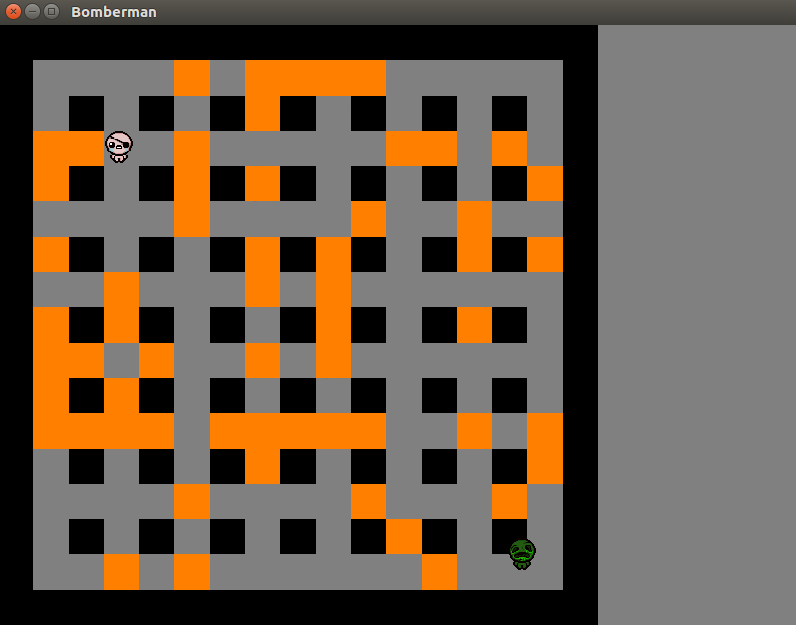
\includegraphics[width=10cm]{jogo}
 \caption{Imagem do jogo}
 \label{im.jogo}
\end{figure}

\subsection{Movimento dos Jogadores}
\label{movimento}
Para criar o movimento dos jogadores foi definido o tipo de dados \texttt{Movimento}:

\begin{verbatim}
data Movimento = Esquerda | Direita | Cima | Baixo | Parado
\end{verbatim}

A cada jogador é atribuído uma lista de \texttt{Movimento}, desta lista será considerado
apenas o 1º elemento para efetuar o movimento dos jogadores na função \texttt{reageTempo}.
No início do jogo, o movimento de cada jogador define-se por \texttt{[Parado]}.
Imaginando que temos dois jogadores, ficaria o 2º elemento do \texttt{Estado} como
\texttt{[(0,[Parado]),(1,[Parado])]}

Sempre que é pressionada uma tecla correspondente ao movimento de um jogador,
este movimento é adicionado à cabeça da lista de movimentos deste jogador.
Se no exemplo anterior o jogador 1 pressionasse seguidamente as teclas para se mover
para cima e para baixo passaríamos a ter \texttt{[(0,[Parado]),(1,[Baixo,Cima,Parado])]}.

Quando uma tecla é largada, o movimento correspondente a essa tecla será eliminado da
lista de movimentos. Caso o jogador 1, no exemplo anterior, largue a tecla para baixo,
iríamos ter \texttt{[(0,[Parado]),(1,[Cima,Parado])]}.

\subsection{Tipo de Câmara}
\label{camara}

Para o desenho do estado do jogo durante o jogo existem 2 opções, cãmara única (Figura \ref{im.jogo})
ou câmaras individuais (Figura \ref{cam.ind}).

Para o desenho com câmaras individuais foi necessário transladar cada câmara pelo simétrico
das coordenadas de cada jogador para que cada jogador tivesse a sua câmara centrada em
si mesmo. Para além disso, reescreveu-se cada função de desenho utilizada pelo tipo de câmara
única para que apenas desenhasse objetos a menos de uma dada distância.
Ainda se achou necessário adicionar uns marcadores. Estes são desenhados quando os
adversários estão demasiado longe.

\begin{figure}[h]
 \centering
 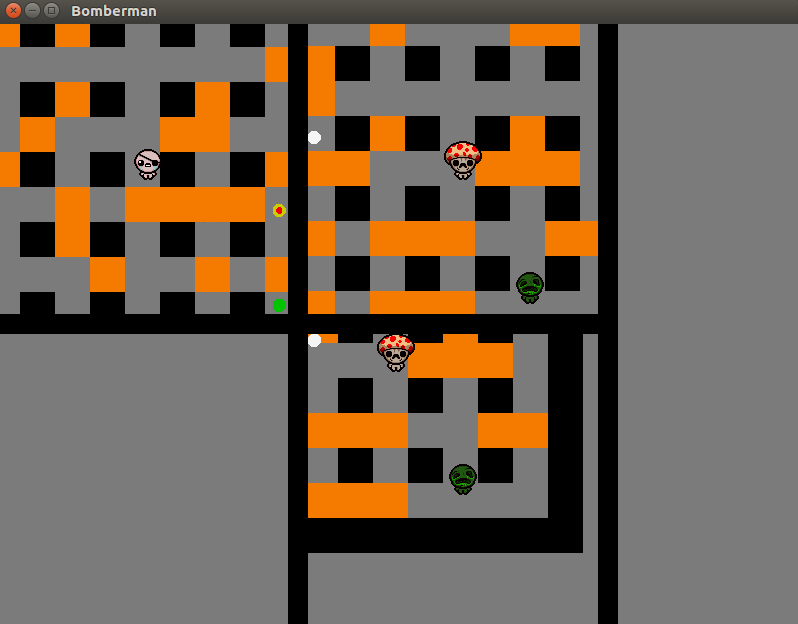
\includegraphics[width=10cm]{cam_ind}
 \caption{Imagem do jogo com câmaras individuais}
 \label{cam.ind}
\end{figure}

\section{Tarefa 6}
\label{tarefa6}

A tarefa 6 consistia na implementação de um \textit{bot} que jogasse Bomberman automaticamente.
A implementação da estratégia passou por definir as seguintes prioridades
(ordem decrescente de prioridade): 
\begin{enumerate}
  \item Manter-se no centro do mapa no fim do jogo
  \item Evitar bombas
  \item Destruir tijolos
  \item Atacar Jogadores
  \item Mover-se para o centro
\end{enumerate}

A 1ª prioridade consiste em manter-se no centro e colocar uma bomba quando
já não é possível explodir bombas antes do tempo acabar. Esta estratégia tem
o objetivo de tentar motivar os adversários a saírem do centro do mapa.

A 2ª prioridade passa por tentar evitar bombas caso elas estejam próximas o
suficiente para causar perigo ao \textit{bot}.

A próxima prioridade é a de por uma bomba para destruir tijolos sempre que o \textit{bot}
esteja adjacente a um tijolo. Com esta estratégia, o \textit{bot} não vai à procura de
tijolos para destruir.

A 4ª prioridade é a de colocar uma bomba caso faltem mais de 30 ticks para o jogo
acabar e exista um jogador adjacente ou na mesma posição que o \textit{bot}. O \textit{bot} deixa de
atacar quando faltam menos de 30 ticks para que tenha tempo de se mover para o
centro do mapa caso seja necessário.

Caso nenhum dos métodos anteriores seja aplicável, o \textit{bot} vai-se movendo até
ao centro do mapa.


\section{Conclusões}
\label{sec:conclusao}

Concluindo, os objetivos das tarefas propostas desta UC e o resultado final foram
de encontro com os objetivos estabelecidos.

\end{document}
